%-*-latex-*-
\sectionthree{Implementation}
\begin{python0}
from solutions import *; clear()
\end{python0}

Frequently heaps are implemented using arrays,
i.e., they are array trees.

%-*-latex-*-

\begin{ex} 
  \label{ex:prob-00}
  \tinysidebar{\debug{exercises/{disc-prob-28/question.tex}}}

  \solutionlink{sol:prob-00}
  \qed
\end{ex} 
\begin{python0}
from solutions import *
add(label="ex:prob-00",
    srcfilename='exercises/discrete-probability/prob-00/answer.tex') 
\end{python0}


%-*-latex-*-

\begin{ex} 
  \label{ex:prob-00}
  \tinysidebar{\debug{exercises/{disc-prob-28/question.tex}}}

  \solutionlink{sol:prob-00}
  \qed
\end{ex} 
\begin{python0}
from solutions import *
add(label="ex:prob-00",
    srcfilename='exercises/discrete-probability/prob-00/answer.tex') 
\end{python0}


There are 2 ways of doing the above.

Method 1:
For object $x$, instead of using $x.priority$,
use $(priority, time)$ where the minheap maintains
a time that is incremented every time
an insert occurs. The ordering of $(priority, time)$
is dictionary.
For the case of maxheap, decrement the time counter.

Disadvantage: If the heap runs for a very long time,
the time might overflow.

Method 2:
The heap is made up of linked list of values.
Each linked list contains values of the same priority.
When a value $x$ is inserted, if $x.priority$ occurs in
the minheap, insert $x$ into the correct linked list.
If x's priority is new, create a new linked list and
insert into heap.
Note that we need to know if a linked list of the
correct priority exists in the heap.
We can have a hash table of (priority, heap index).
During heap operations (heapify-up and -down), the
hash table must be updated during the swaps.
If the root linked list is empty, it is removed from the heap.
If the heap allows priority modification, then
a non-root linked list can become empty -- this should not be
delete.
Therefore during the extract-root operation,
need to loop over the extract-root operation until
the new root is a non-empty linked list.

%-*-latex-*-

\begin{ex} 
  \label{ex:prob-00}
  \tinysidebar{\debug{exercises/{disc-prob-28/question.tex}}}

  \solutionlink{sol:prob-00}
  \qed
\end{ex} 
\begin{python0}
from solutions import *
add(label="ex:prob-00",
    srcfilename='exercises/discrete-probability/prob-00/answer.tex') 
\end{python0}


Clearly the following must work: copy constructor, destructor,
\verb!operator=!, \verb!operator==!.
The class should look like this:
\begin{console}
template < typename T >
class MaxHeap
{
public:
private:
    std::vector < T > x;
};
\end{console}

%-*-latex-*-

\begin{ex} 
  \label{ex:prob-00}
  \tinysidebar{\debug{exercises/{disc-prob-28/question.tex}}}

  \solutionlink{sol:prob-00}
  \qed
\end{ex} 
\begin{python0}
from solutions import *
add(label="ex:prob-00",
    srcfilename='exercises/discrete-probability/prob-00/answer.tex') 
\end{python0}


\section{Non-array implementation}

For a non-array implementation of heaps,
consider this:


\begin{center}

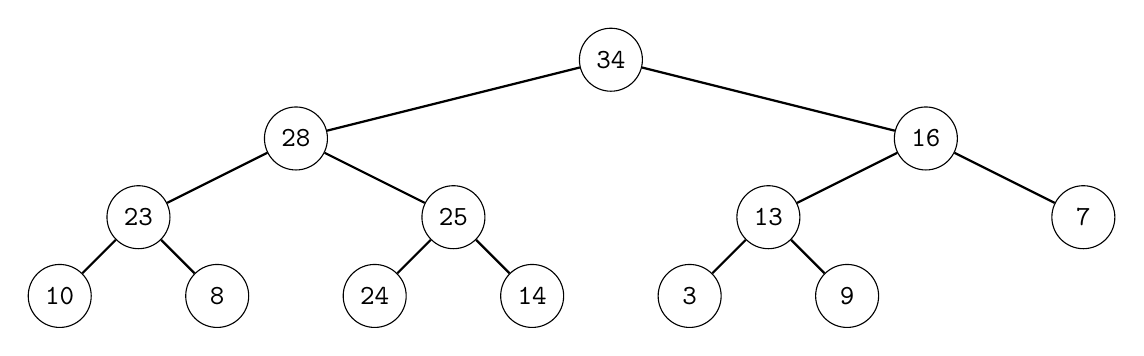
\begin{tikzpicture}
\node at (7,-1) [circle,draw,minimum size=8mm] (A) {\texttt{34}};
\node at (3,-2) [circle,draw,minimum size=8mm] (B) {\texttt{28}};
\node at (11,-2) [circle,draw,minimum size=8mm] (C) {\texttt{16}};
\node at (1,-3) [circle,draw,minimum size=8mm] (D) {\texttt{23}};
\node at (5,-3) [circle,draw,minimum size=8mm] (E) {\texttt{25}};
\node at (9,-3) [circle,draw,minimum size=8mm] (F) {\texttt{13}};
\node at (13,-3) [circle,draw,minimum size=8mm] (G) {\texttt{7}};
\node at (0,-4) [circle,draw,minimum size=8mm] (H) {\texttt{10}};
\node at (2,-4) [circle,draw,minimum size=8mm] (I) {\texttt{8}};
\node at (4,-4) [circle,draw,minimum size=8mm] (J) {\texttt{24}};
\node at (6,-4) [circle,draw,minimum size=8mm] (K) {\texttt{14}};
\node at (8,-4) [circle,draw,minimum size=8mm] (L) {\texttt{3}};
\node at (10,-4) [circle,draw,minimum size=8mm] (M) {\texttt{9}};
\draw [-,thick] (A) -- (B);
\draw [-,thick] (A) -- (C);
\draw [-,thick] (B) -- (D);
\draw [-,thick] (B) -- (E);
\draw [-,thick] (C) -- (G);
\draw [-,thick] (C) -- (F);
\draw [-,thick] (D) -- (H);
\draw [-,thick] (D) -- (I);
\draw [-,thick] (E) -- (J);
\draw [-,thick] (E) -- (K);
\draw [-,thick] (F) -- (L);
\draw [-,thick] (F) -- (M);

;
\end{tikzpicture}
    
\end{center}



Of course I need a pointer to the root.
That's pretty obvious.
Another thing to note is that because of the way I add nodes,
i.e., always at the lowest level and left-to-right, I should have a pointer
to the parent where I have a new node.

%-*-latex-*-

\begin{ex} 
  \label{ex:prob-00}
  \tinysidebar{\debug{exercises/{disc-prob-28/question.tex}}}

  \solutionlink{sol:prob-00}
  \qed
\end{ex} 
\begin{python0}
from solutions import *
add(label="ex:prob-00",
    srcfilename='exercises/discrete-probability/prob-00/answer.tex') 
\end{python0}


However that takes $(\log n)$ time.
So we might as well have a pointer that records where the
insert should go.
But that's not enough.
Once a level is full, we need to go to the next level.
Therefore we need two (and not one) extra pointer.
Like this:

\begin{center}
\begin{tikzpicture}


\node at (7,-1) [circle,draw,minimum size=8mm] (A) {\texttt{34}};
\node at (3,-2) [circle,draw,minimum size=8mm] (B) {\texttt{28}};
\node at (11,-2) [circle,draw,minimum size=8mm] (C) {\texttt{16}};
\node at (1,-3) [circle,draw,minimum size=8mm] (D) {\texttt{23}};
\node at (5,-3) [circle,draw,minimum size=8mm] (E) {\texttt{25}};
\node at (9,-3) [circle,draw,minimum size=8mm] (F) {\texttt{13}};
\node at (13,-3) [circle,draw,minimum size=8mm] (G) {\texttt{7}};
\node at (0,-4) [circle,draw,minimum size=8mm] (H) {\texttt{10}};
\node at (2,-4) [circle,draw,minimum size=8mm] (I) {\texttt{8}};
\node at (4,-4) [circle,draw,minimum size=8mm] (J) {\texttt{24}};
\node at (6,-4) [circle,draw,minimum size=8mm] (K) {\texttt{14}};
\node at (8,-4) [circle,draw,minimum size=8mm] (L) {\texttt{3}};
\node at (10,-4) [circle,draw,minimum size=8mm] (M) {\texttt{9}};
\node at (12,-4) [circle,draw,minimum size=8mm] (N) {\texttt{5}};
\draw [-,thick] (A) -- (B);
\draw [-,thick] (A) -- (C);
\draw [-,thick] (B) -- (D);
\draw [-,thick] (B) -- (E);
\draw [-,thick] (C) -- (G);
\draw [-,thick] (C) -- (F);
\draw [-,thick] (D) -- (H);
\draw [-,thick] (D) -- (I);
\draw [-,thick] (E) -- (J);
\draw [-,thick] (E) -- (K);
\draw [-,thick] (F) -- (L);
\draw [-,thick] (F) -- (M);
\draw [-,thick] (G) -- (N);

;

    \node (proot) at (7,0.5) {\texttt{proot}} ;\path [-triangle 60] (proot) edge[] (A);\node (p0) at (1,-4.5) {\texttt{p0}} ;\path [-triangle 60] (p0) edge[] (D);\node (p1) at (13,-4.5) {\texttt{p1}} ;\path [-triangle 60] (p1) edge[] (G);\node (p) at (13,-1.5) {\texttt{p}} ;\path [-triangle 60] (p) edge[] (G);
\end{tikzpicture}

\end{center}



Note that each node has not just left child and right child pointer.
When we do delete, we might need to go to the previous level.
That means that each node must have a parent pointer too.
Of course the parent pointer is also needed when I do heapify-up, right?

If I insert \texttt{4} to the above, then I get this:

\begin{center}
\begin{tikzpicture}

\fill[white] (0.0, 0.0) circle (0.3);
\node [line width=0.03cm,black,minimum size=0.57cm,draw,circle] at (0.0,0.0)(8){};\draw (0.0, 0.0) node[color=black] {\texttt{8}};
\fill[white] (-2.8, -1.0) circle (0.3);
\node [line width=0.03cm,black,minimum size=0.57cm,draw,circle] at (-2.8,-1.0)(5){};\draw (-2.8, -1.0) node[color=black] {\texttt{5}};
\fill[white] (2.8, -1.0) circle (0.3);
\node [line width=0.03cm,black,minimum size=0.57cm,draw,circle] at (2.8,-1.0)(15){};\draw (2.8, -1.0) node[color=black] {\texttt{15}};
\fill[white] (-4.2, -2.0) circle (0.3);
\node [line width=0.03cm,black,minimum size=0.57cm,draw,circle] at (-4.2,-2.0)(3){};\draw (-4.2, -2.0) node[color=black] {\texttt{3}};
\fill[white] (-1.4, -2.0) circle (0.3);
\node [line width=0.03cm,black,minimum size=0.57cm,draw,circle] at (-1.4,-2.0)(6){};\draw (-1.4, -2.0) node[color=black] {\texttt{6}};
\fill[white] (1.4, -2.0) circle (0.3);
\node [line width=0.03cm,black,minimum size=0.57cm,draw,circle] at (1.4,-2.0)(10){};\draw (1.4, -2.0) node[color=black] {\texttt{10}};
\fill[white] (4.2, -2.0) circle (0.3);
\node [line width=0.03cm,black,minimum size=0.57cm,draw,circle] at (4.2,-2.0)(22){};\draw (4.2, -2.0) node[color=black] {\texttt{22}};
\fill[white] (-3.5, -3.0) circle (0.3);
\node [line width=0.03cm,black,minimum size=0.57cm,draw,circle] at (-3.5,-3.0)(4){};\draw (-3.5, -3.0) node[color=black] {\texttt{4}};
\fill[white] (0.7, -3.0) circle (0.3);
\node [line width=0.03cm,black,minimum size=0.57cm,draw,circle] at (0.7,-3.0)(9){};\draw (0.7, -3.0) node[color=black] {\texttt{9}};
\fill[white] (2.1, -3.0) circle (0.3);
\node [line width=0.03cm,black,minimum size=0.57cm,draw,circle] at (2.1,-3.0)(12){};\draw (2.1, -3.0) node[color=black] {\texttt{12}};
\fill[white] (3.5, -3.0) circle (0.3);
\node [line width=0.03cm,black,minimum size=0.57cm,draw,circle] at (3.5,-3.0)(18){};\draw (3.5, -3.0) node[color=black] {\texttt{18}};
\fill[white] (4.9, -3.0) circle (0.3);
\node [line width=0.03cm,black,minimum size=0.57cm,draw,circle] at (4.9,-3.0)(28){};\draw (4.9, -3.0) node[color=black] {\texttt{28}};
\fill[white] (3.15, -4.0) circle (0.3);
\node [line width=0.03cm,black,minimum size=0.57cm,draw,circle] at (3.15,-4.0)(17){};\draw (3.15, -4.0) node[color=black] {\texttt{17}};
\fill[white] (3.8500000000000005, -4.0) circle (0.3);
\node [line width=0.03cm,black,minimum size=0.57cm,draw,circle] at (3.8500000000000005,-4.0)(19){};\draw (3.8500000000000005, -4.0) node[color=black] {\texttt{19}};\draw[line width=0.03cm,black,->,>=triangle 60] (8) to  (5);
\draw[line width=0.03cm,black,->,>=triangle 60] (8) to  (15);
\draw[line width=0.03cm,black,->,>=triangle 60] (5) to  (3);
\draw[line width=0.03cm,black,->,>=triangle 60] (5) to  (6);
\draw[line width=0.03cm,black,->,>=triangle 60] (15) to  (10);
\draw[line width=0.03cm,black,->,>=triangle 60] (15) to  (22);
\draw[line width=0.03cm,black,->,>=triangle 60] (3) to  (4);
\draw[line width=0.03cm,black,->,>=triangle 60] (10) to  (9);
\draw[line width=0.03cm,black,->,>=triangle 60] (10) to  (12);
\draw[line width=0.03cm,black,->,>=triangle 60] (22) to  (18);
\draw[line width=0.03cm,black,->,>=triangle 60] (22) to  (28);
\draw[line width=0.03cm,black,->,>=triangle 60] (18) to  (17);
\draw[line width=0.03cm,black,->,>=triangle 60] (18) to  (19);
\end{tikzpicture}

\end{center}



If I add \texttt{8}, I get this:

\begin{center}
\begin{tikzpicture}

\fill[white] (0.0, 0.0) circle (0.3);
\node [line width=0.03cm,black,minimum size=0.57cm,draw,circle] at (0.0,0.0)(6){};\draw (0.0, 0.0) node[color=black] {\texttt{6}};
\fill[white] (-2.8, -1.0) circle (0.3);
\node [line width=0.03cm,black,minimum size=0.57cm,draw,circle] at (-2.8,-1.0)(5){};\draw (-2.8, -1.0) node[color=black] {\texttt{5}};
\fill[white] (2.8, -1.0) circle (0.3);
\node [line width=0.03cm,black,minimum size=0.57cm,draw,circle] at (2.8,-1.0)(15){};\draw (2.8, -1.0) node[color=black] {\texttt{15}};
\fill[white] (-4.2, -2.0) circle (0.3);
\node [line width=0.03cm,black,minimum size=0.57cm,draw,circle] at (-4.2,-2.0)(3){};\draw (-4.2, -2.0) node[color=black] {\texttt{3}};
\fill[white] (1.4, -2.0) circle (0.3);
\node [line width=0.03cm,black,minimum size=0.57cm,draw,circle] at (1.4,-2.0)(10){};\draw (1.4, -2.0) node[color=black] {\texttt{10}};
\fill[white] (4.2, -2.0) circle (0.3);
\node [line width=0.03cm,black,minimum size=0.57cm,draw,circle] at (4.2,-2.0)(22){};\draw (4.2, -2.0) node[color=black] {\texttt{22}};
\fill[white] (-3.5, -3.0) circle (0.3);
\node [line width=0.03cm,black,minimum size=0.57cm,draw,circle] at (-3.5,-3.0)(4){};\draw (-3.5, -3.0) node[color=black] {\texttt{4}};
\fill[white] (0.7, -3.0) circle (0.3);
\node [line width=0.03cm,black,minimum size=0.57cm,draw,circle] at (0.7,-3.0)(9){};\draw (0.7, -3.0) node[color=black] {\texttt{9}};
\fill[white] (2.1, -3.0) circle (0.3);
\node [line width=0.03cm,black,minimum size=0.57cm,draw,circle] at (2.1,-3.0)(12){};\draw (2.1, -3.0) node[color=black] {\texttt{12}};
\fill[white] (3.5, -3.0) circle (0.3);
\node [line width=0.03cm,black,minimum size=0.57cm,draw,circle] at (3.5,-3.0)(18){};\draw (3.5, -3.0) node[color=black] {\texttt{18}};
\fill[white] (4.9, -3.0) circle (0.3);
\node [line width=0.03cm,black,minimum size=0.57cm,draw,circle] at (4.9,-3.0)(28){};\draw (4.9, -3.0) node[color=black] {\texttt{28}};
\fill[white] (3.15, -4.0) circle (0.3);
\node [line width=0.03cm,black,minimum size=0.57cm,draw,circle] at (3.15,-4.0)(17){};\draw (3.15, -4.0) node[color=black] {\texttt{17}};
\fill[white] (3.8500000000000005, -4.0) circle (0.3);
\node [line width=0.03cm,black,minimum size=0.57cm,draw,circle] at (3.8500000000000005,-4.0)(19){};\draw (3.8500000000000005, -4.0) node[color=black] {\texttt{19}};\draw[line width=0.03cm,black,->,>=triangle 60] (6) to  (5);
\draw[line width=0.03cm,black,->,>=triangle 60] (6) to  (15);
\draw[line width=0.03cm,black,->,>=triangle 60] (5) to  (3);
\draw[line width=0.03cm,black,->,>=triangle 60] (15) to  (10);
\draw[line width=0.03cm,black,->,>=triangle 60] (15) to  (22);
\draw[line width=0.03cm,black,->,>=triangle 60] (3) to  (4);
\draw[line width=0.03cm,black,->,>=triangle 60] (10) to  (9);
\draw[line width=0.03cm,black,->,>=triangle 60] (10) to  (12);
\draw[line width=0.03cm,black,->,>=triangle 60] (22) to  (18);
\draw[line width=0.03cm,black,->,>=triangle 60] (22) to  (28);
\draw[line width=0.03cm,black,->,>=triangle 60] (18) to  (17);
\draw[line width=0.03cm,black,->,>=triangle 60] (18) to  (19);
\end{tikzpicture}

\end{center}



Once I add a \texttt{9}, I get this:

\begin{center}
\begin{tikzpicture}


\node at (8,-1) [circle,draw,minimum size=8mm] (A) {\texttt{34}};
\node at (4,-2) [circle,draw,minimum size=8mm] (B) {\texttt{28}};
\node at (12,-2) [circle,draw,minimum size=8mm] (C) {\texttt{16}};
\node at (2,-3) [circle,draw,minimum size=8mm] (D) {\texttt{23}};
\node at (6,-3) [circle,draw,minimum size=8mm] (E) {\texttt{25}};
\node at (10,-3) [circle,draw,minimum size=8mm] (F) {\texttt{13}};
\node at (14,-3) [circle,draw,minimum size=8mm] (G) {\texttt{7}};
\node at (1,-4) [circle,draw,minimum size=8mm] (H) {\texttt{10}};
\node at (3,-4) [circle,draw,minimum size=8mm] (I) {\texttt{8}};
\node at (5,-4) [circle,draw,minimum size=8mm] (J) {\texttt{24}};
\node at (7,-4) [circle,draw,minimum size=8mm] (K) {\texttt{14}};
\node at (9,-4) [circle,draw,minimum size=8mm] (L) {\texttt{3}};
\node at (11,-4) [circle,draw,minimum size=8mm] (M) {\texttt{9}};
\node at (13,-4) [circle,draw,minimum size=8mm] (N) {\texttt{5}};
\node at (15,-4) [circle,draw,minimum size=8mm] (O) {\texttt{4}};
\node at (0,-5) [circle,draw,minimum size=8mm] (P) {\texttt{8}};
\node at (2,-5) [circle,draw,minimum size=8mm] (Q) {\texttt{9}};
\draw [-,thick] (A) -- (B);
\draw [-,thick] (A) -- (C);
\draw [-,thick] (B) -- (D);
\draw [-,thick] (B) -- (E);
\draw [-,thick] (C) -- (G);
\draw [-,thick] (C) -- (F);
\draw [-,thick] (D) -- (H);
\draw [-,thick] (D) -- (I);
\draw [-,thick] (E) -- (J);
\draw [-,thick] (E) -- (K);
\draw [-,thick] (F) -- (L);
\draw [-,thick] (F) -- (M);
\draw [-,thick] (G) -- (N);
\draw [-,thick] (G) -- (O);
\draw [-,thick] (H) -- (P);
\draw [-,thick] (H) -- (Q);

;

    \node (proot) at (8,0.5) {\texttt{proot}} ;\path [-triangle 60] (proot) edge[] (A);\node (p0) at (1,-5.5) {\texttt{p0}} ;\path [-triangle 60] (p0) edge[] (H);\node (p1) at (15,-5.5) {\texttt{p1}} ;\path [-triangle 60] (p1) edge[] (O);\node (p1) at (3,-5.5) {\texttt{p}} ;\path [-triangle 60] (p1) edge[] (I);
\end{tikzpicture}

\end{center}



Get it?

  
Clearly the above idea works for complete trees where
nodes are added left-to-right at the last level.

Note that \verb!p! points to the parent where new nodes should be
attached but does not have information on whether it should be
as a left or as a right child.
You can also include an integer variable \texttt{num\_children}
to tell you how many children
there are.
If the number of children is 0, then the new node should be
attached as a left child.
If the number of children is 1, then the new node should be attached
as a right child.

%-*-latex-*-

\begin{ex} 
  \label{ex:prob-00}
  \tinysidebar{\debug{exercises/{disc-prob-28/question.tex}}}

  \solutionlink{sol:prob-00}
  \qed
\end{ex} 
\begin{python0}
from solutions import *
add(label="ex:prob-00",
    srcfilename='exercises/discrete-probability/prob-00/answer.tex') 
\end{python0}


%-*-latex-*-

\begin{ex} 
  \label{ex:prob-00}
  \tinysidebar{\debug{exercises/{disc-prob-28/question.tex}}}

  \solutionlink{sol:prob-00}
  \qed
\end{ex} 
\begin{python0}
from solutions import *
add(label="ex:prob-00",
    srcfilename='exercises/discrete-probability/prob-00/answer.tex') 
\end{python0}

